\section*{Formation personnalis�e Serveur Linux}

\subsection*{D�tails pratiques}

\begin{minipage}[l]{.5\linewidth}

	\raggedright
	\begin{itemize}
		\item Dur�e : \textbf{2 Jours}

		\item Lieu : Marseille

		\item D�tails : Fin Mai 2017 / D�but juin 2017

		\item Horaires : 9h-12h30 et 14h-17h30

		\item Repas midi : inclus

		\item H�tels : liste disponible sur demande

		\item R�servations : email. formations@evolix.fr\\
			\hspace*{2.2cm} tel. 04.91.05.92.54
	\end{itemize}

\end{minipage} \hfill \begin{minipage}[c]{.4\linewidth}	

	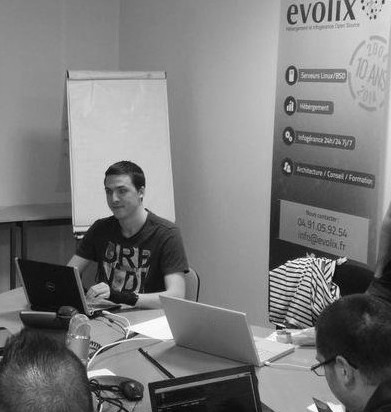
\includegraphics[width=70mm]{./evoformation}

\end{minipage}

\subsection*{Objectifs}

\begin{itemize}
	\item Installer un serveur Linux
	\item S�curiser un syst�me Linux
	\item Administrer Linux
	\item Configurer et administrer Apache
	\item Configurer et administrer PostgreSQL
\end{itemize}

\subsection*{Pr�-requis}

\begin{itemize}
	\item Notions d'administration syst�me et r�seau
	\item Connaissance des commandes Unix de base
	\item Bases d'architecture des ordinateurs
	\item Bases d'anglais
\end{itemize}
